
\subsection{Dataset}
\paragraph*{Data composition and preprocess}
The sequence is represented by the symbol of amino acids such as L, K, M, etc., typically 7-50
in length. Specially, we use 1 to represent the oxidation of methionine (M), and we use 2,3,4 to represent the phosphorylation of serine(S), threonine(T), tyrosine(Y), respectively. And those representation is also used in the Ion Intensity task.

% Retention time (RT) is a measure of the time taken for a solute to pass through a chromatography column.
% It is calculated as the time from injection to detection.
For RT datasets, they are comprised of pairs of
\( \{X, y\} \). $X:= \{ <x_1, x_2, x_3,\dots, x_n> \}$, $x_i$
is amino acid,and \( y \) is the retention time. 
To train a better model, we first sequentially pre-train the models in four datasets called 
For building the virtual library, we split the dataset into train : validation = 9 : 1,
selecting the best model on validation set; for model comparison, the dataset is split into train : validation : test
= 8 : 1 : 1, reporting results on the test set.

As the retention time is distributed in the real-world unit, such as minutes or seconds, we scale each dataset by its max and min of retention time to 0 - 1 by the following formula. To cover all RT dataset distributions, we set the max(RT) as 200, and min(RT) as -100.

In further, we support the peptide with N-terminal acetyl modification. We use the * symbol to indicate modification, @ to indicate no modification. We pad all sequences to the length of the longest sequence in the dataset to form a matrix feeding into the neural network.

Like RT dataset, the ion intensity datasets are comprised of pairs of
\( \{X, y\} \). $X := \{ <x_1, x_2, x_3,\dots, x_i, \dots, x_n, +q> \}$, $x_i$ is amino acid, $+q$
is the charge carried by the
peptide sequence before it is fragmented in the mass spectrometer. And \( y \) is the spectrum of the peptide. Each y is composed of pairs of key and value.
The key is the ion's name, such as y2+1, b6+2, and the value is their corresponding raw intensity.
We divide each intensity by the maximum of the intensities within a peptide sequence to normalize each intensity into 0-1. As kinds of ions in the dataset is severely imbalanced, we only select the 8 types of ions same as pdeep2~\cite{zeng2019ms}, that is
b(y)i+1-noloss, b(y)i+2-noloss, b(y)i+1-1,H3PO4 and b(y)i+2-1,H3PO4, i indicating the site of b(y)ion,
to feed the neural network and predict those 8 types of ion intensity. Those ion intensities are formed as the matrix of shape 8 * length of the sequence (illustrated in the supplementary).
There are two types of fragment ion intensity values that have no contribution in the loss calculation and are removed in the prediction. One is that related to padding, like y20 for a 7-mer; the other is related to the phosphorylation site. For example, the phosphorylation site is located in the b5, then the b1,b2, b3, and b4 ions cannot lose phosphate so that the ion intensity with phosphate loss must be 0. This ignorance of impossible phosphorylation site potentially help model to learn the implicitly rule of phosphorylation, benefiting the prediction accuracy of intensity of ion with phosphate loss. Otherwise, the only way for model to learn this rule is from the ion intensity data which would be much more inefficient than the injecting the prior knowledge directly to the model learning.
The data split, N-terminal acetyl modification indicator and padding operation are the same as the RT dataset.


\paragraph*{Metric}
\subsubsection*{RT}
The $\Delta$$t_{95\%}$ metric is used as the main metric, which represents
the minimal time window containing the deviations between observed and predicted RTs for 95\% of
the peptides.
\[ \Delta t_{95\%} = 2 * | y - \hat{y} |_{95\%} \]
The subscript 95\% means the 95\% rank of the deviations.
We select the model by $\Delta$$t_{95\%}$ metric.
Pearson Correlation Coefficient (PCC) is also referred.
\subsubsection*{Ion Intensity}
We compute each peptide's PCC and select the median of those PCCs as the final evaluation metric.
Primarily, we follow Prosit~\cite{gessulat2019prosit} using normalized
spectral angle(SA) as another metric and the median of those SAs is reported as the final evaluation result.
SA's formula is as follows:

\[ SA = 1 - 2 * \frac{cos^{-1}(\hat{V_a}\cdot\hat{V_b})}{\pi} \]
$\hat{V}$ is a vector whose L2 norm equals 1. We select the model by the median PCC metric.

\subsection{RT experiments}
For this task, we compare results of two datasets of our model with DeepRT and different model architecture setting, the performance
is shown in table \ref{table:Human}, Figure \ref{fig:Human_results} and table \ref{table:Jeff}, Figure \ref{fig:Jeff_results}. We could see that we use the
half number of parameters of DeepRT but achieve better performance in two datasets. And our model's prediction could
fit the real RT distribution very well.



%\begin{figure}[t]
%
%   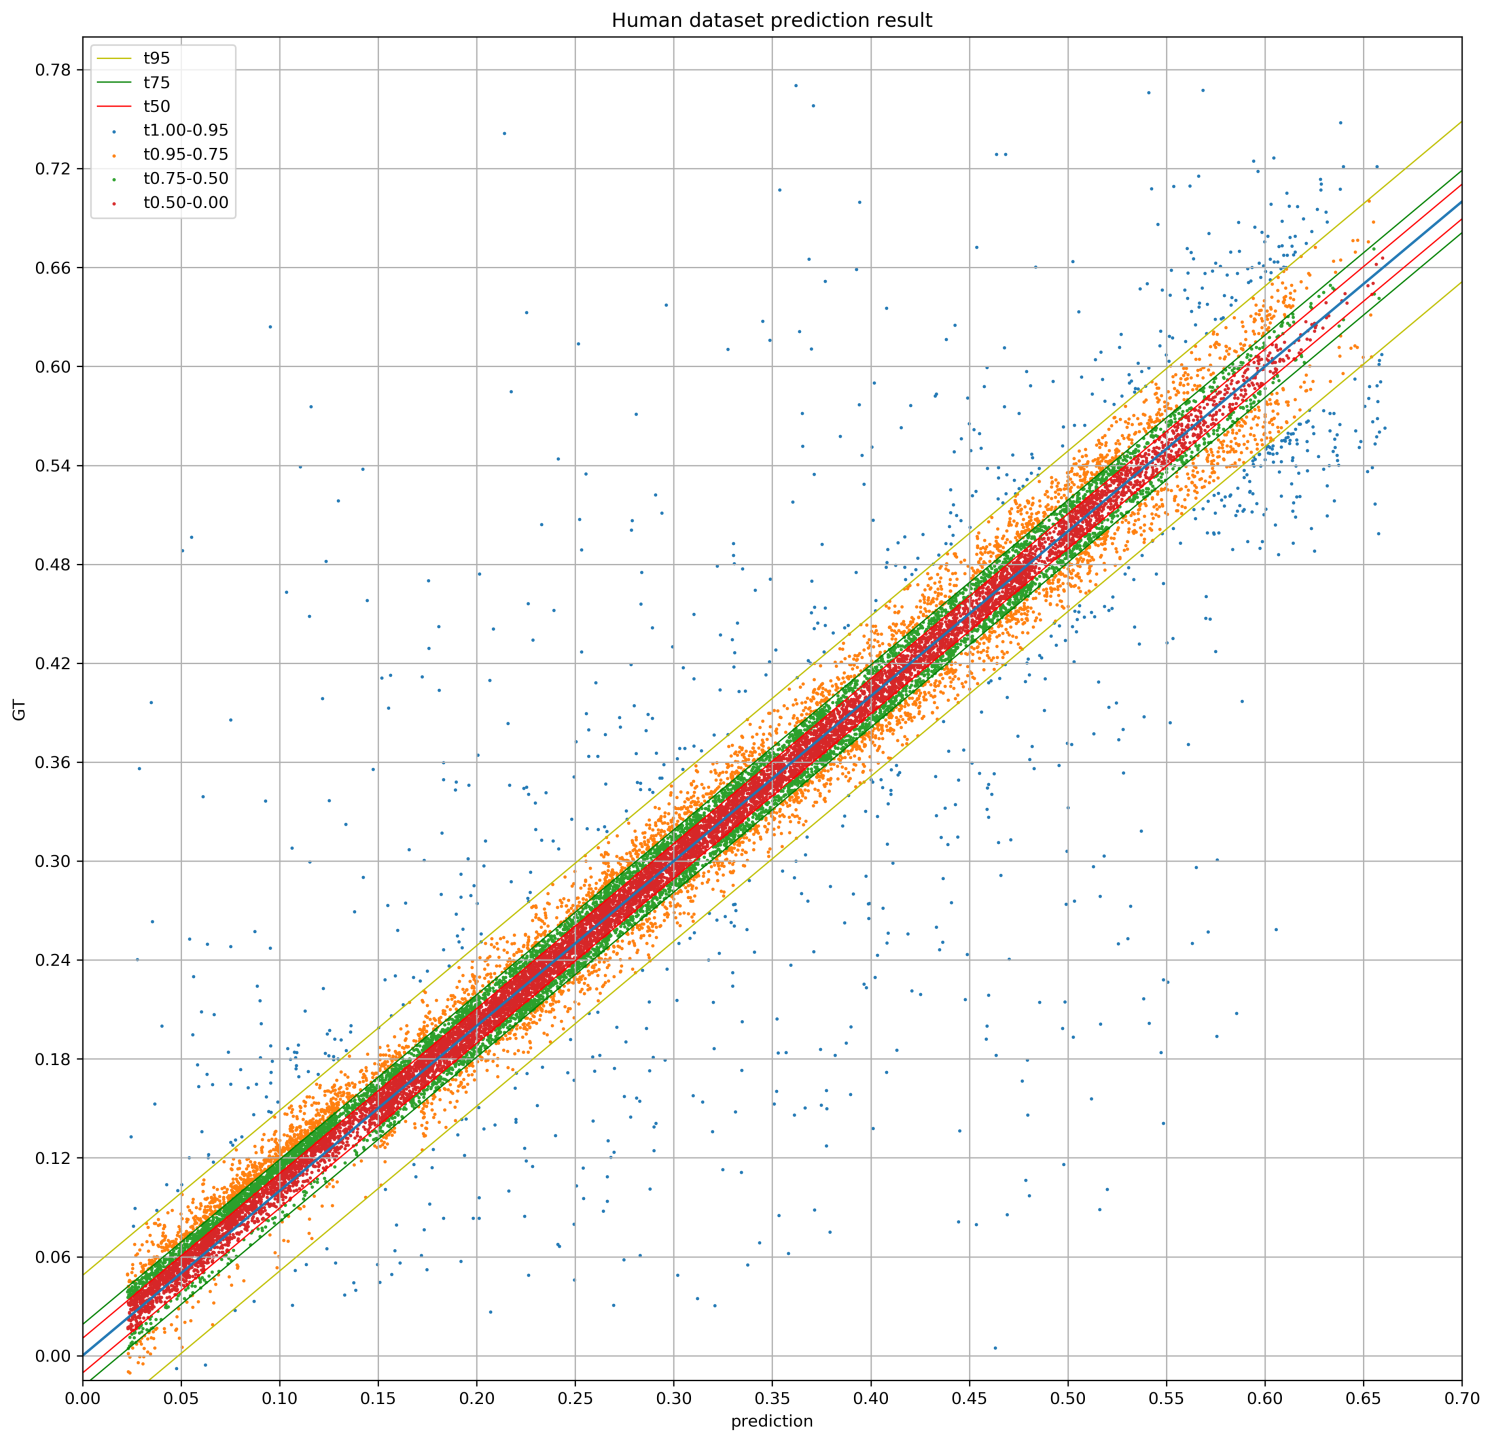
\includegraphics[width=3.0in]{Human_results}
%
%   \caption{Visualization of human dataset}
%% \label{fig:long}
%\label{fig:Human_results}
%\end{figure}
%
%\begin{figure}[t]
%
%   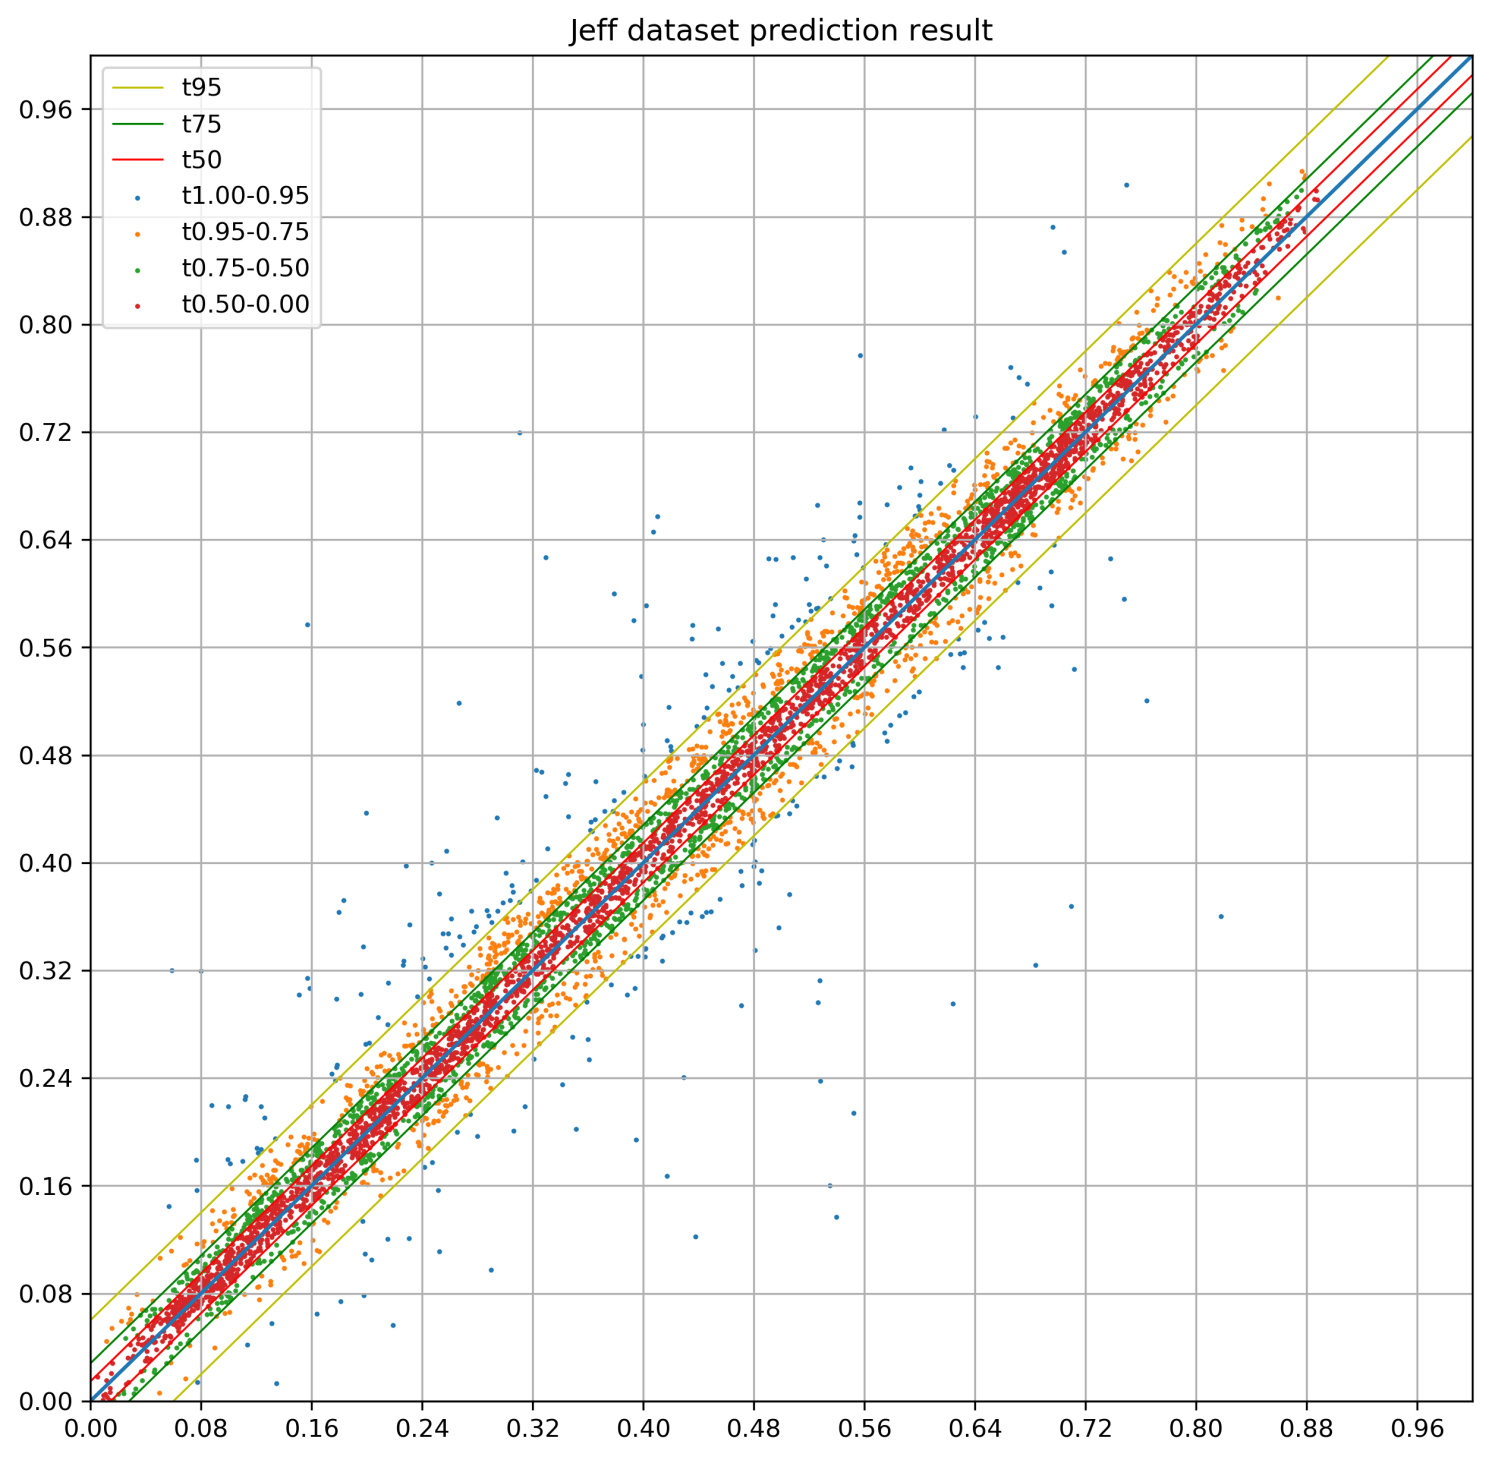
\includegraphics[width=3.0in]{Jeff_results}
%
%   \caption{Visualization of Jeff dataset}
%\label{fig:Jeff_results}
%\end{figure}

\subsection{Ion Intensity experiments}
As we have explore the architecture in the RT task, so that we only compare with the pdeep2.
The DDA comparison is shown in Figure \ref{fig:DDA}, Table \ref{table:DDA} and Figure \ref{fig:DIA18},
Table \ref{table:DIA18}.
From the results, we could see that in the metric median PCC and SA, we have beaten the SOTA model
pdeep2. In further, to explain our model's good generalization ability, we train our model in the DDA
dataset and direct test on the DIA18 dataset. Results are show in the Figure \ref{fig:DIA18_direct} and Table \ref{table:DIA18_direct}.
And we could see results that model trained on the DDA dataset, test on DIA18 dataset are comparable to trained
on DIA18, and are even similar to pdeep2's results on DIA18.
%-------------------------------------------------------------------------

\subsection{ablation study}
%\begin{figure}[t]
%
%   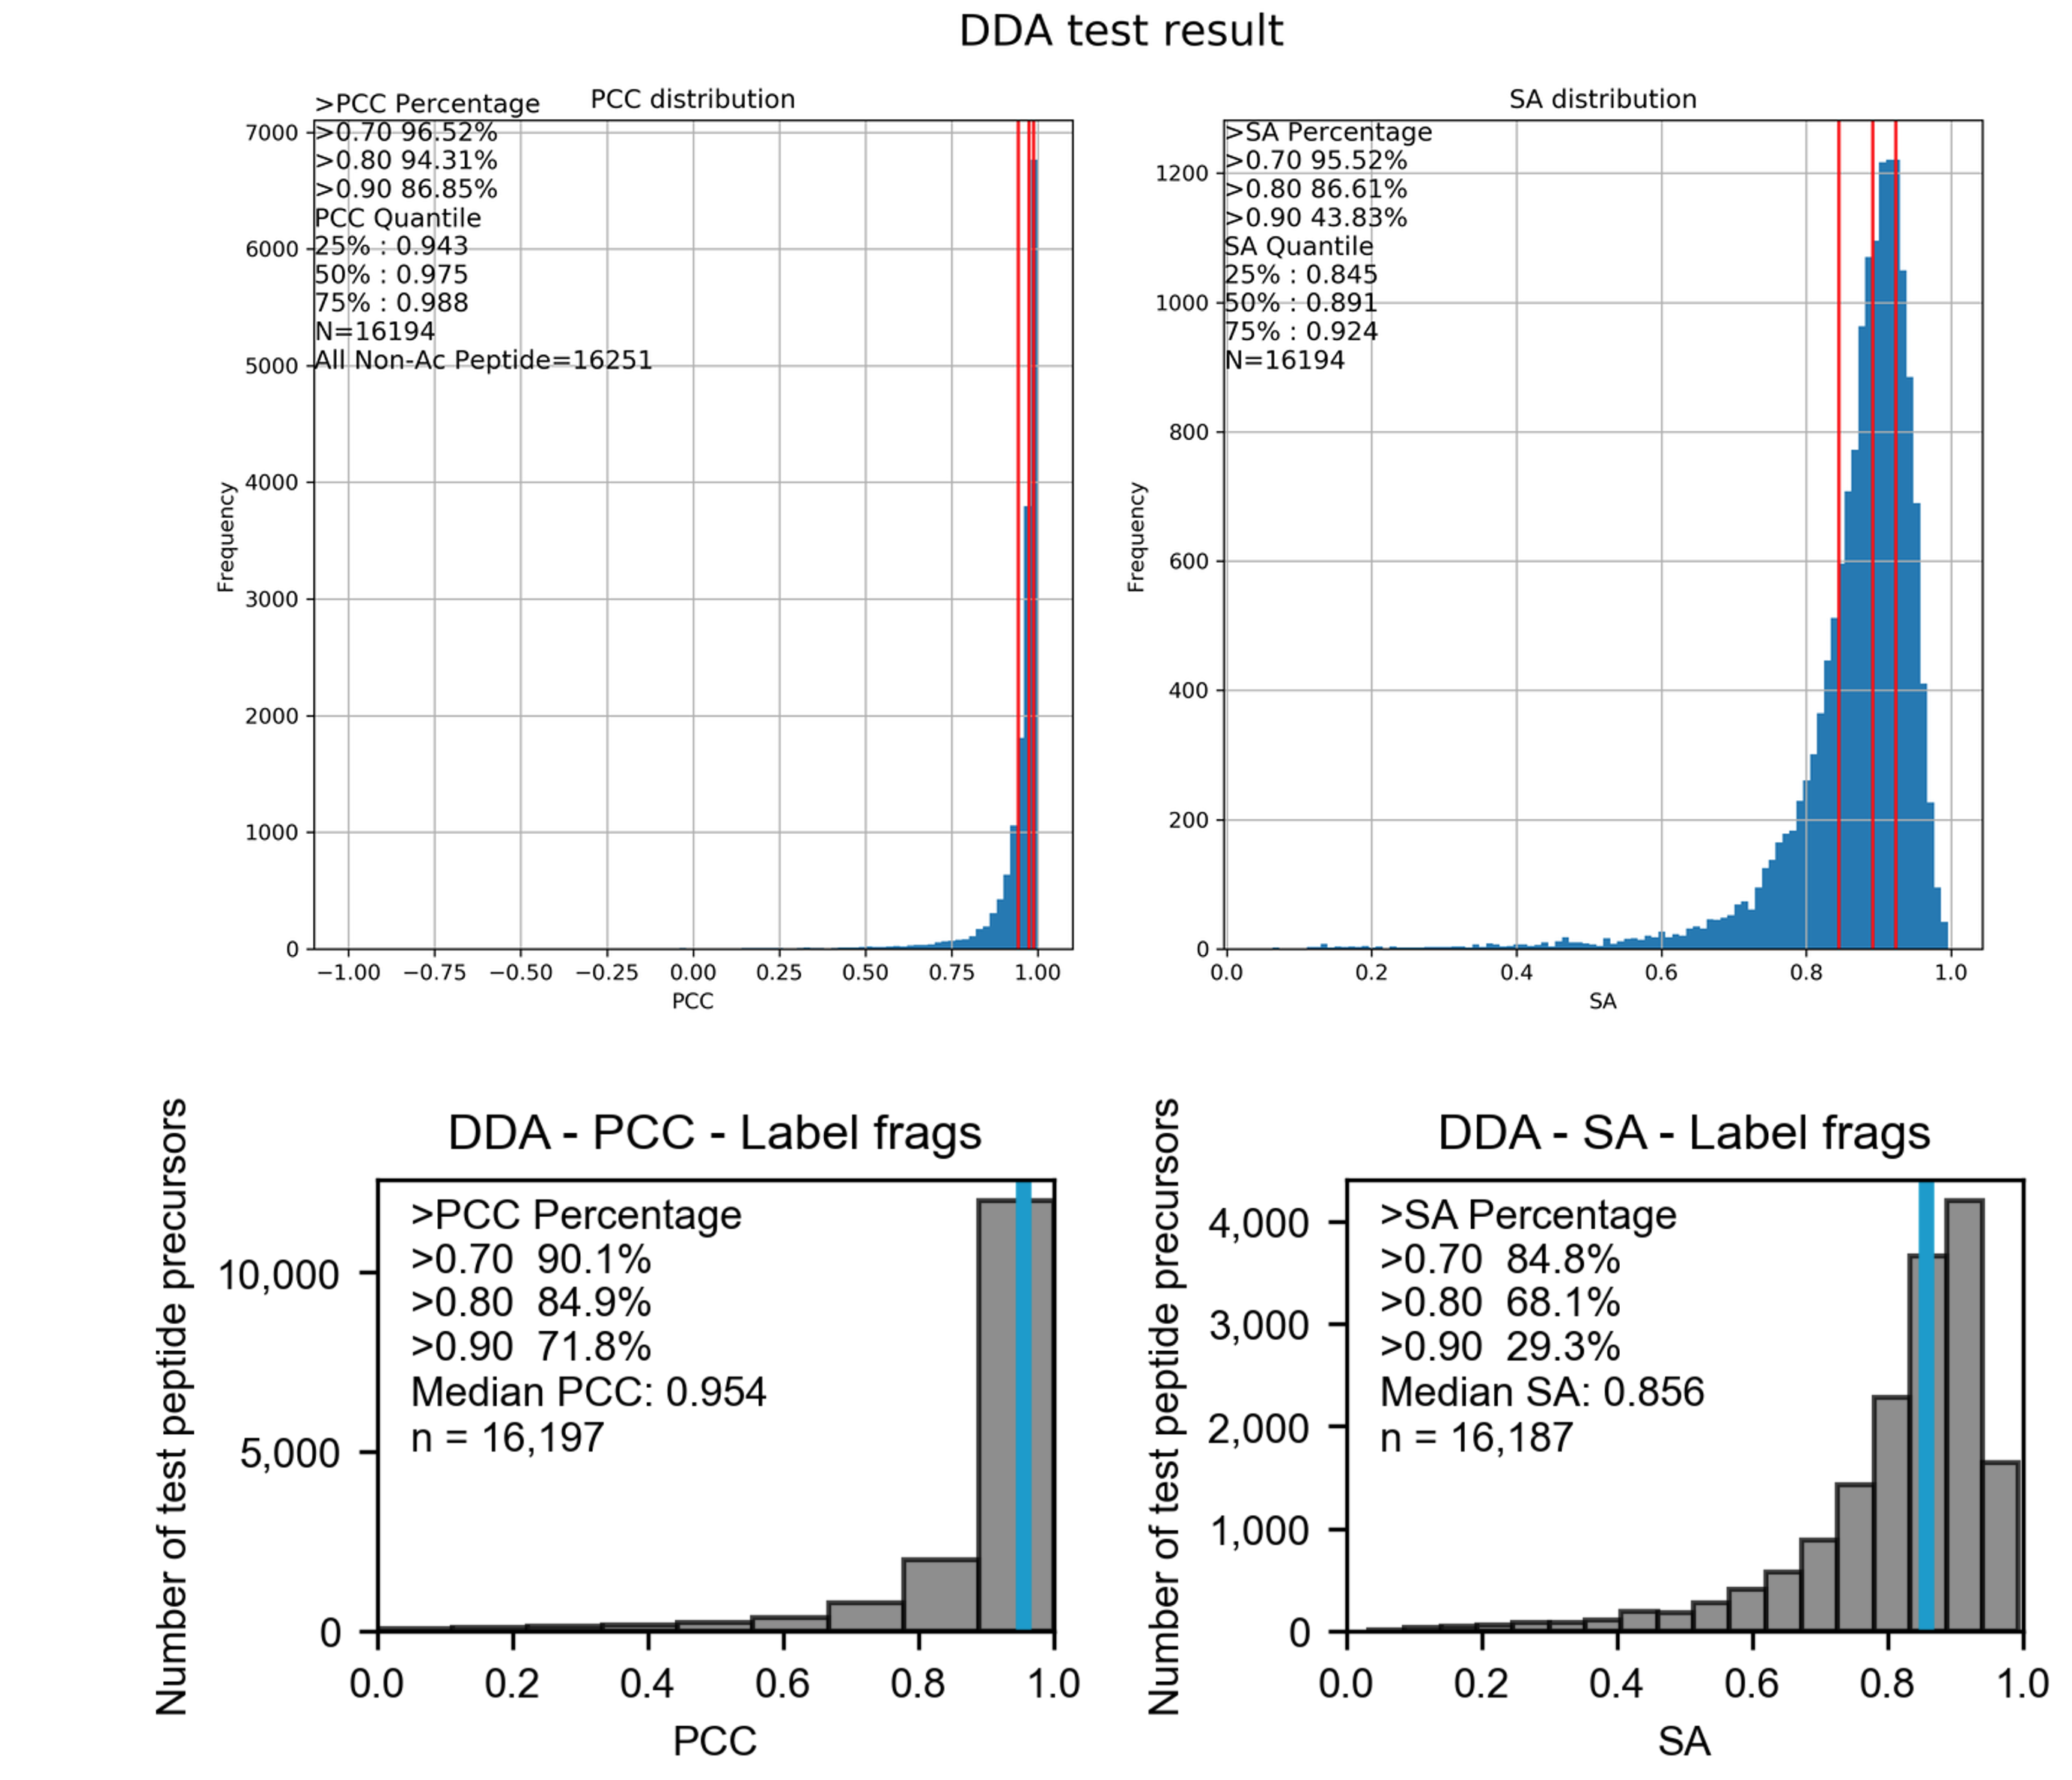
\includegraphics[width=3.0in]{DDA}
%
%   \caption{Visualization of performance of DDA dataset. The above is ours and the below is pdeep2}
%\label{fig:DDA}
%\end{figure}
%
%
%\begin{figure}[t]
%
%   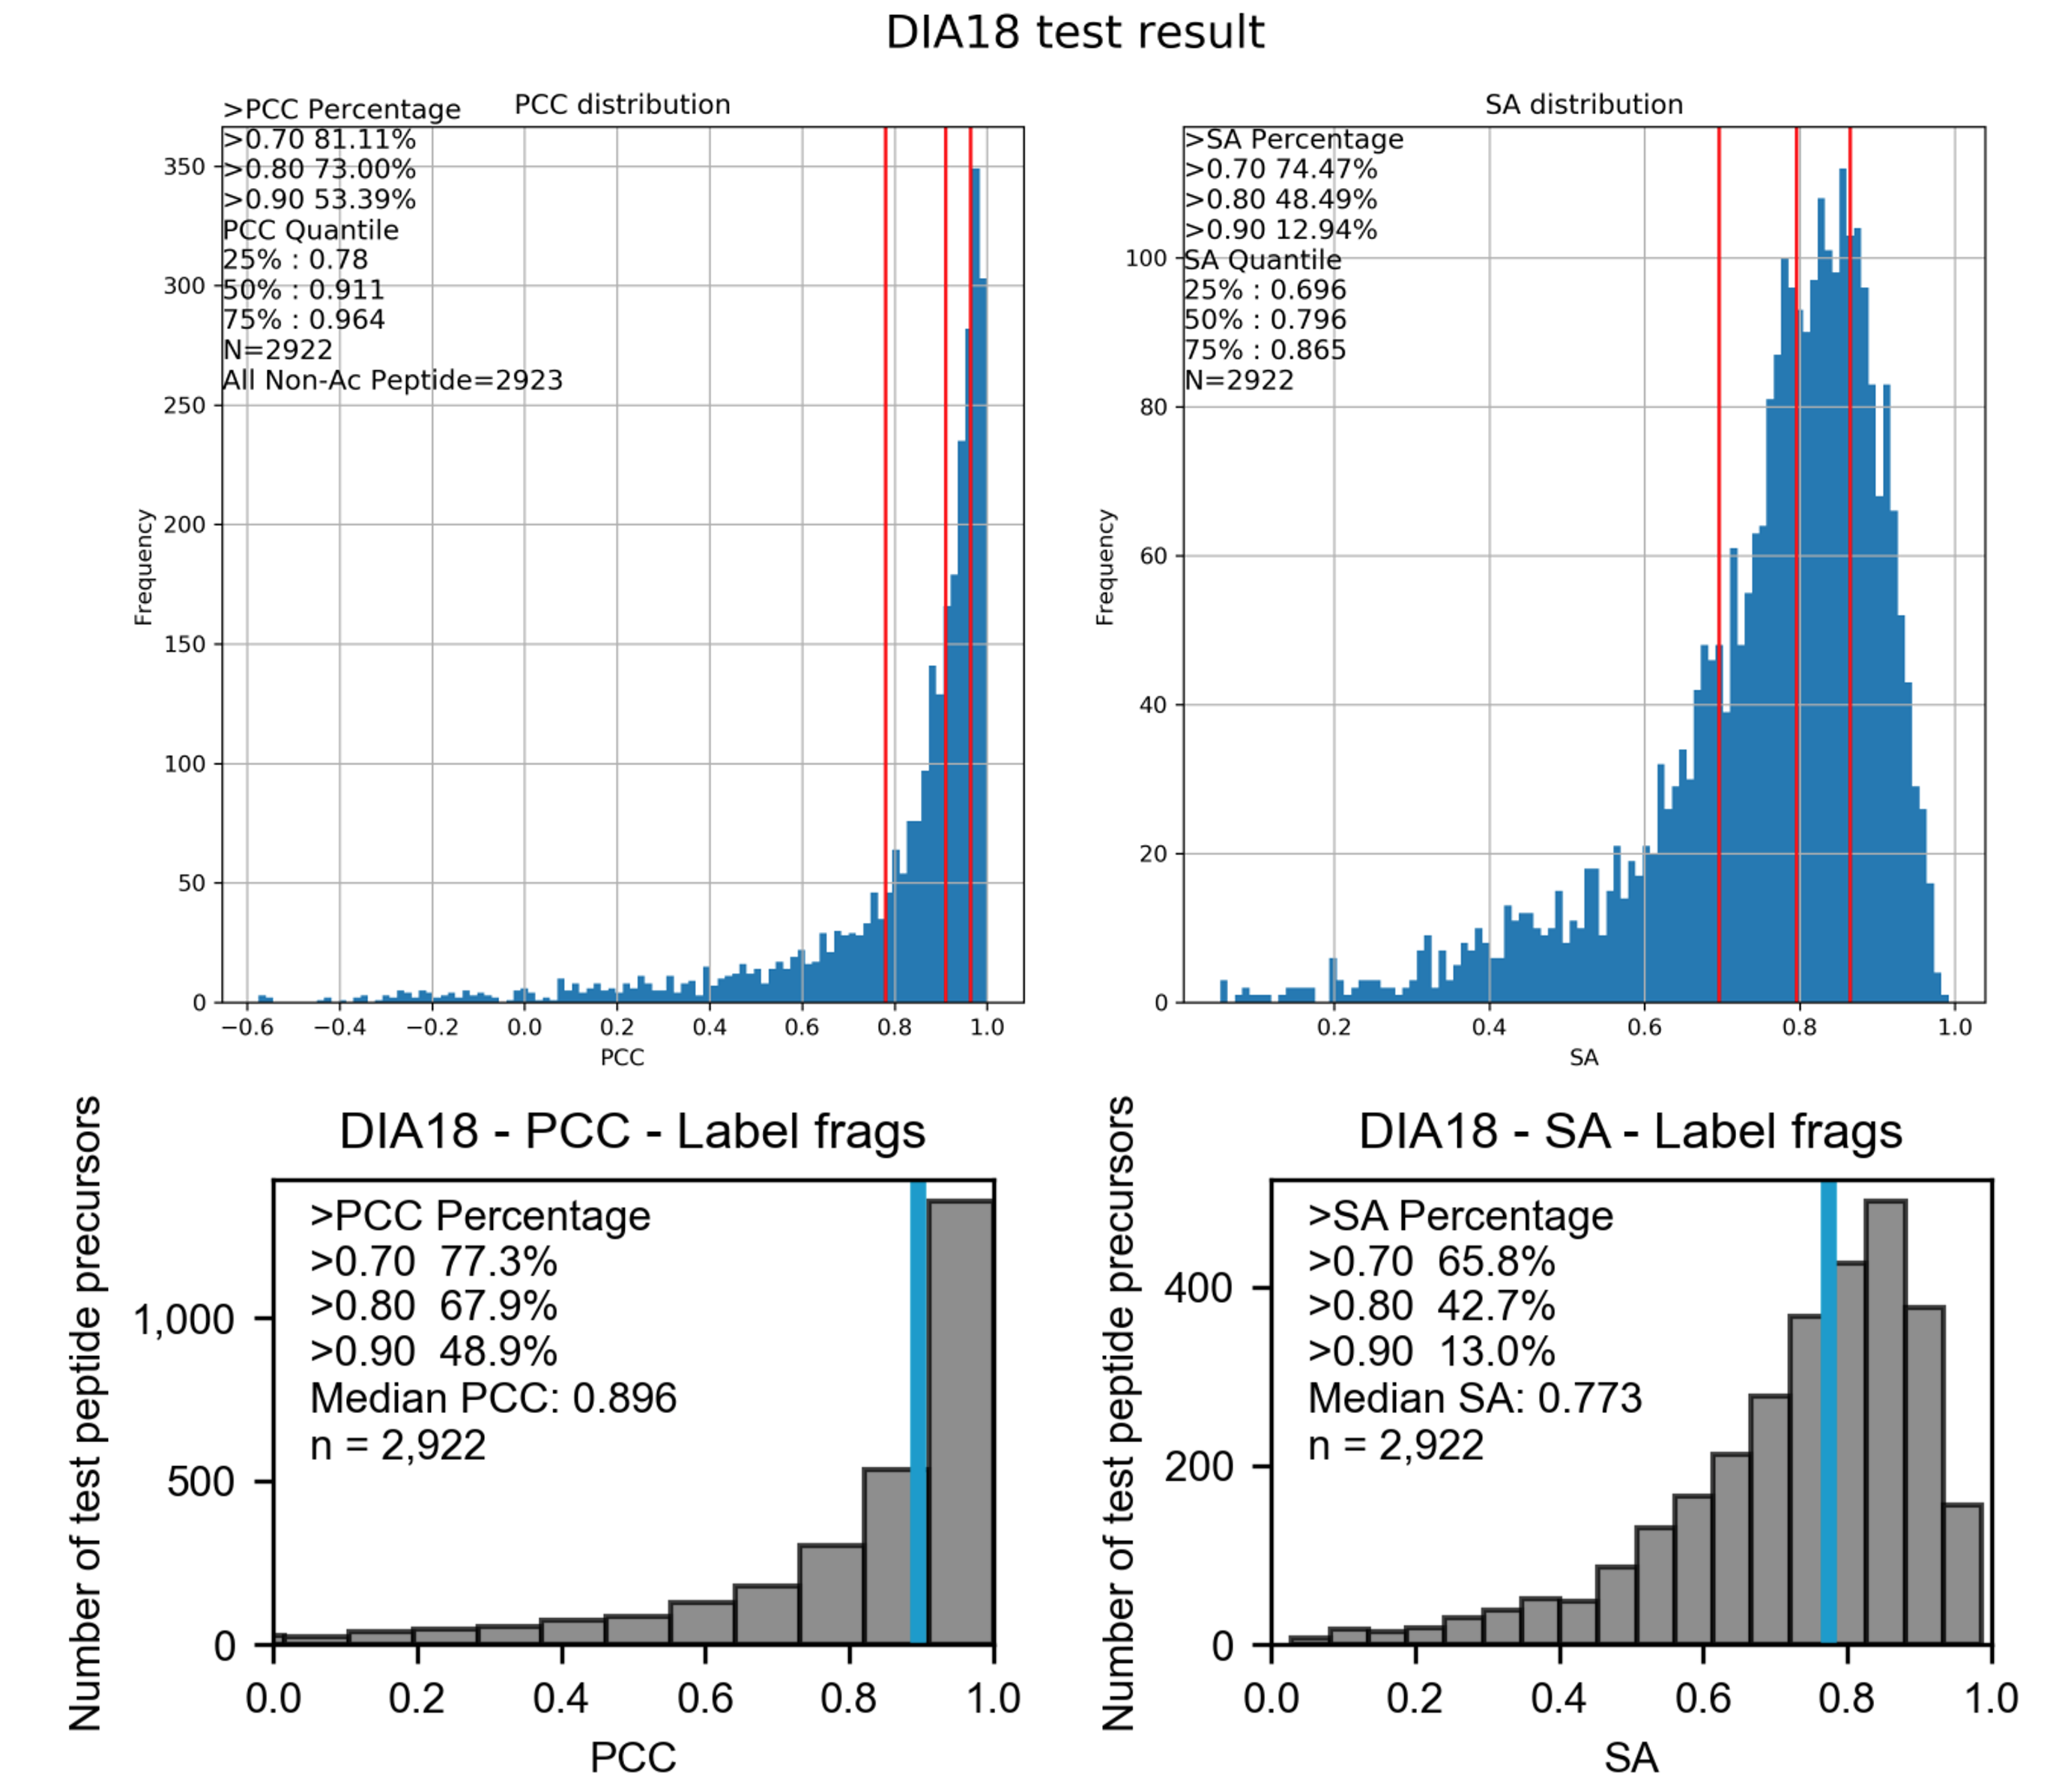
\includegraphics[width=3.0in]{DIA18}
%
%   \caption{Visualization of DIA18 dataset. The above is ours and the below is pdeep2}
%\label{fig:DIA18}
%\end{figure}
%
%
%\begin{figure}[t]
%
%   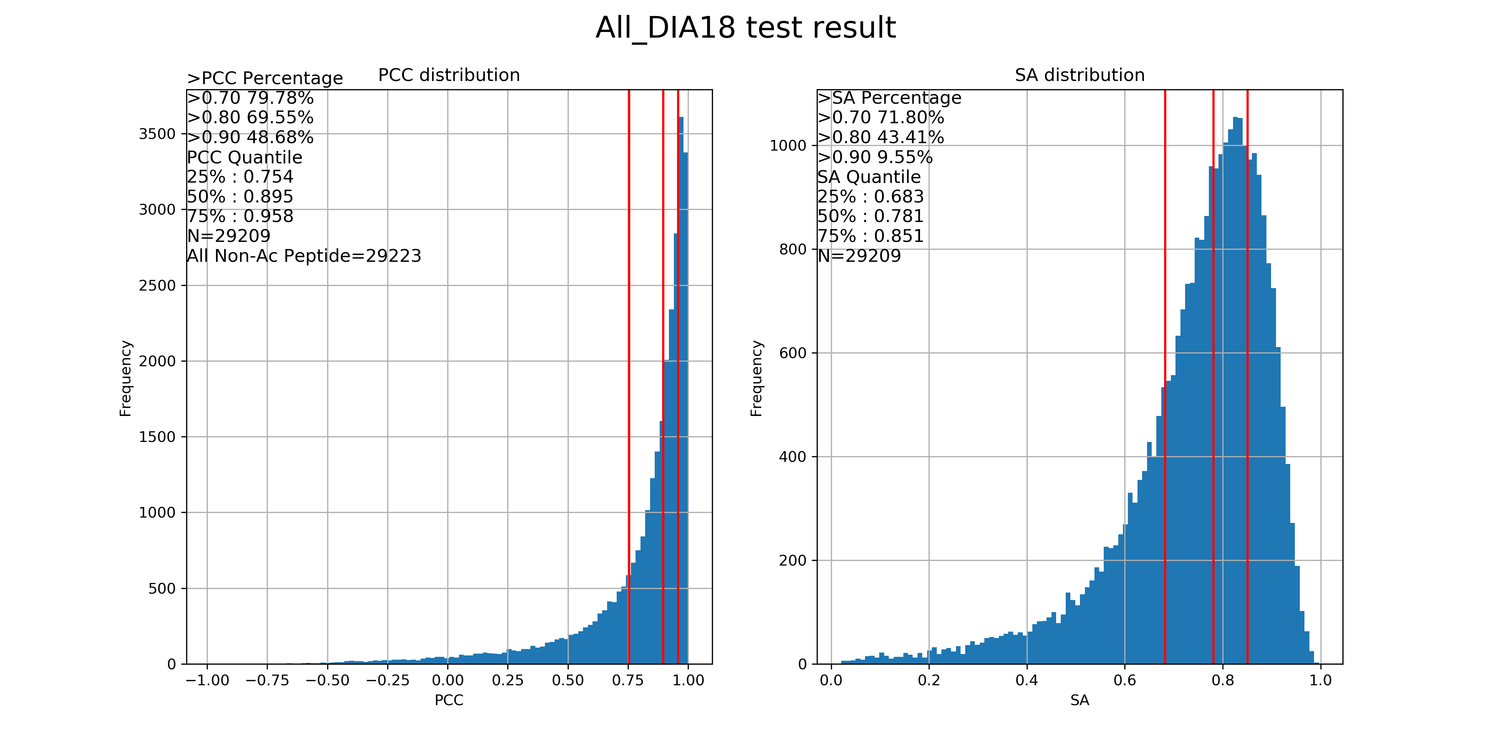
\includegraphics[width=3.5in]{DIA_direct_test}
%
%   \caption{Direct test on DIA18 dataset.}
%\label{fig:DIA18_direct}
%\end{figure}
%

\begin{table}
   \begin{center}
   \begin{tabularx}{\columnwidth}{|Y|Y|}
   \hline
   data description & no. of peptides \\
   \hline
   HumanPhosDB~\cite{lawrence2016plug} & 204560 \\
   Jeff~\cite{liu2018vivo} & 67,552 \\
   VeroE6~\cite{bouhaddou2020global} & 43,407  \\
   R2P2~\cite{leutert2019r2} & 35,810 \\
   U2OS-DIA~\cite{wang2020naguider} & 48,329\\
   RPE1-DIA~\cite{bekker2020rapid} & 33,578  \\
   RPE1-DDA~\cite{bekker2020rapid} & 129,111  \\
   \hline
   \end{tabularx}
   \end{center}
   \caption{Retention time pretraining datasets}
   \label{table:pretrained_Dataset}
   \end{table}

\begin{table}
   \begin{center}
   \begin{tabular}{|l|c|c|}
   \hline
   Model & $\Delta$$t_{95\%}$ & parameters \\
   \hline\hline
   DeepRT & 15.67 & 3.1M \\
   LSTM & 14.73 & 1.1M \\
   DeepPhospho & 14.70 & 1.5M \\
   transformer & 17.00 & 3M \\
   \hline
   \end{tabular}
   \end{center}
   \caption{Human Dataset results. Ours is better.}
   \label{table:Human}
   \end{table}


   \begin{table}
      \begin{center}
      \begin{tabular}{|l|c|c|}
      \hline
      Model & $\Delta$$t_{95\%}$ & parameters \\
      \hline\hline
      DeepRT & 19.7 & 3.1M \\
      LSTM & 17.6 & 1.1M \\
      DeepPhospho & 17.3 & 1.5M \\
      transformer & 20.8 & 3M \\
      \hline
      \end{tabular}
      \end{center}
      \caption{Jeff Dataset results.   Ours is better.}
      \label{table:Jeff}
      \end{table}

\begin{table}
   \begin{center}
   \begin{tabular}{|l|c|c|}
   \hline
   Model & Median PCC & Median SA \\
   \hline\hline
   pdeep2 & 0.954 & 0.856 \\
   DeepPhospho$\star$ & 0.975 & 0.891 \\
   \hline
   \end{tabular}
   \end{center}
   \caption{DDA Dataset results.Ours is better.}
   \label{table:DDA}
   \end{table}

\begin{table}
   \begin{center}
   \begin{tabular}{|l|c|c|}
   \hline
   Model & Median PCC & Median SA \\
   \hline\hline
   pdeep2 & 0.896 & 0.773 \\
   DeepPhospho$\star$ & 0.911 & 0.796 \\
   \hline
   \end{tabular}
   \end{center}
   \caption{DIA18 Dataset results.Ours is better.}
   \label{table:DIA18}
\end{table}

\begin{table}
   \begin{center}
   \begin{tabular}{|l|c|c|}
   \hline
   Model & Median PCC & Median SA \\
   \hline\hline
   Direct Test & 0.895 & 0.781 \\
   Train then Test & 0.911 & 0.796 \\
   \hline
   \end{tabular}
   \end{center}
   \caption{DIA18 Dataset results. Direct test only drops little compared to training and test}
   \label{table:DIA18_direct}
\end{table}
%%-------------------------------------------------------------------------